\section{Elektrospinnen mit zwei Düsen}

Das Elektrospinnen ist ein verfahren zur Herstellung komplexer Endlosfasern, welche Durchmesser von wenigen Mikrometern bis hinzu einigen Nanometern ermöglicht. Zum erzeugen der Faser wird eine Schmelze oder Lösung des zu verziehenden Materials benötigt. Diese wird durch eine Düse gefördert, welche zugleich die Elektrode ist. Gegenüber der Elektrode ist mit einem Abstand von circa 10-25cm eine Gegenelektrode positioniert. Zwischen den zwei Elektroden wird eine Hochspannung angelegt, welche ein Elektrisches Feld mit einer Stärke von 100-500 $\frac{kV}{m}$ erzeugt. Durch die Spannung verformt sich der Tropfen am Austrittspunkt der Düse zu einem Konus. Wird die Spannung nun noch weiter erhöht tritt ein Strahl aus der Schmelze aus,welcher als "Jet" bezeichnet wird. Auf dem Weg zur Gegenelektrode verjüngt sich die Faser und härtet aus \cite{Greiner.2007}. Dieses einfache Grundprinzip lässt sich adaptieren um bimorphe Fasern herzustellen. Dazu werden nun die Düsengeometrien angepasst um die Faser dem Anwendungszweck gerecht zu modellieren. 



 \begin{figure}[!h]
     \centering
     \begin{subfigure}[]{.28\textwidth}
         \centering
         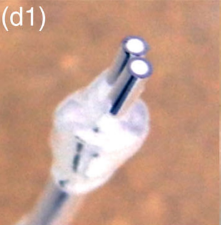
\includegraphics[width=\textwidth]{Abbildungen/side-by-side.png}
         \caption{side-by-side Spinndüse \vspace{3.9mm}}
         \label{fig:side-by-side}
     \end{subfigure}
     \hspace{5mm}
     \begin{subfigure}[]{.285\textwidth}
         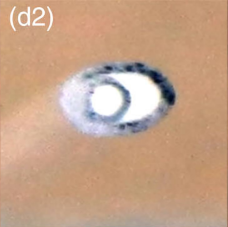
\includegraphics[width=\textwidth]{Abbildungen/acentric_sideby-side.png}
         \caption{Unzentrische side-by-side \\ Spinndüse}
         \label{fig:acentric_sideby-side}
     \end{subfigure}
     \hspace{5mm}
     \begin{subfigure}[]{.29\textwidth}
        \centering
        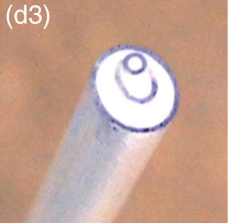
\includegraphics[width=\textwidth]{Abbildungen/a_coaxial_spinneret_with_an_acentric_core.png}
         \caption{Koaxial Spinndüse mit  unzentrischem Kern}
         \label{fig:a_coaxial_spinneret_with_an_acentric_core}
     \end{subfigure}
     \caption{Spinndüsengeometrien \cite{Yu.2020}}
      \label{fig:spinnduesengeometrien}
        \end{figure}

Die in Abbildung \ref{fig:spinnduesengeometrien} dargestellten Formen hätten das Potential eine Faser zu erzeugen die vom Aufbau den Anforderungen entspricht. Aufgrund der Verfahrensweise ist jedoch mit diversen Problemen zu rechnen.  \\
Das wichtigste ist das die Verwendeten Flüssigkeiten miteinander kompatibel sind und so das Spinnen einer Faser ermöglichen. Um dies festzustellen gibt es vier Merkmale die erfüllt sein sollten. Als erstes darf keins der Fluide die Fähigkeit besitzen die Düsen zu verstopfen. Zweitens ist es wichtig das zwischen den Flüssigkeiten weder chemische noch physikalische Reaktionen auftreten und das es zwischen den Lösungen kein großes Konzentrationsgefälle gibt, da eine Diffusion die Spinnfähigkeit beeinflusst. Als letztes ist es wichtig das die Kräfte an den Grenzflächen so gering wie möglich sind\cite{Yu.2020}.
Diese enge Abhängigkeit von Geometrie und Materialeigenschften und deren Wechselwirkungen macht das verfahren recht unflexibel. Weiterhin ist der Produzierbare Dimensionumfang der Fasern sehr gering was die Einsetzbarkeit einschränkt. Das größte Manko ist jedoch das nur Fluide verarbeitet werden können. Im gewünschten Anwendungsbereich führt das dazu das ein schnelles und flexibles Ausprobieren verschiedenster Materialkombination schwierig wäre.


\section{Thermisches Faserziehen} \label{sec:therm}
%verfahren aus den Veröffentlichungen (gestaltung der preform)

Das Thermische Faserziehen ist eine relativ gut erforschte Technik und wird vor allem in der Informationstechnik angewandt. Dieses Verfahren wird zum Beispiel zur Herstellung von optischen Fasern, wie Glasfasern, verwendet. Zumeist werden so nur Fasern aus einem Material hergestellt, wobei sich das Prinzip zur Herstellung von bimorphen Fasern kaum unterscheidet. Abbildung \ref{fig:thermal_fiber_drawing} zeigt den 

\begin{wrapfigure}{l}{0.6\textwidth}
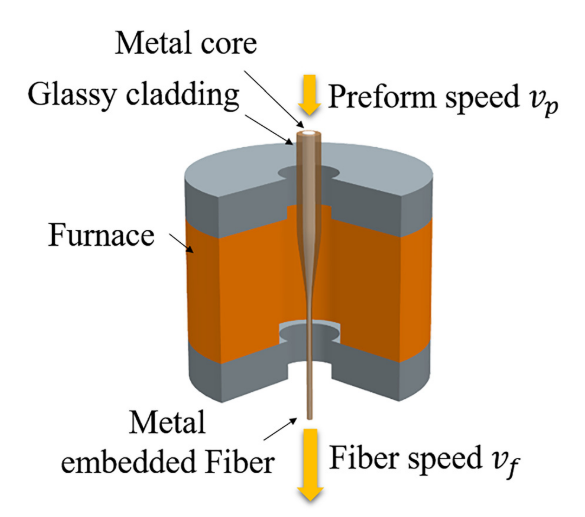
\includegraphics[width=0.9\linewidth]{Abbildungen/Schematic_of_thermal_fiber_drawing.png} 
\caption{Schematischer Aufbau thermisches Ziehen \cite{Zhao.2016}}
\label{fig:thermal_fiber_drawing}
\end{wrapfigure}

Schematischen Aufbau des Prozesses, bei welchem in  eine Faser aus Metall hergestellt wird. Bevor eine Faser gezogen werden kann muss zunächst die Preform hergestellt werden. Verwendet wird ein Bündel aus mehreren Strängen \ac{sn} , welche in einem Mantel aus \ac{pes} eingebracht werden. Wichtig ist dabei das der Mantel eine möglicht gut kontrollierbare Viskosität beim erwärmen vorweist. Weiterhin sollte die Materialkombination so gewählt sein das der Kern während des Prozesses Schmelzen, also eine ähnliche Schmelztemperatur wie der Mantel besitzt. Wenn nun die Materialien während des Erwärmens nicht miteinander Reagieren sollte eine verzugsbereite Multimaterial-Preform vorliegen. Während des  im ofen sollte die Preform aufgrund ihres Eigengewichtes eine Verjüngung ausbilden. Wird nun an der Faser gezogen kann mittels Gleichung \ref{eq:dicke_faser_zhao} die Dicke der abgezogenen Faser variiert werden\cite{Zhao.2016}.
\begin{equation}
    \frac{v_f}{v_p} = \frac{D_p^2}{D_f^2} 
    \label{eq:dicke_faser_zhao}
\end{equation}
Der große Vorteil dieses Verfahrens ist die Möglichkeit vielfältig Preformen einfach und schnell auszuprobieren. Dabei ist zu beachten, das die Preformen, nicht auf einen Runden Querschnitt limitiert sind, sondern das auch andere Symetrisch aufgebaute Ausgangsformen denkbar sind. Einzig das Abschmelzverhalten der einzelnen Materialen ist schwer vorherzusagen und sollte in einzelnen versuchen untersucht werden. 
In verschieden anderen Veröffentlichungen wurde dieses Verfahren ebenfalls verwendet um Sensor und Aktorgarne herzustellen, was die Anwendbarkeit für das vorliegende Problem bestätigt\cite{Kanik.2019}\cite{Leber.2023}.
Für den Fall das sich dieses Verfahren bewährt ist der Prozess auch gut Skalierbar und würde sich so für ein Industrielle Fertigung eignen.
